\section{Fotometría}

Para este trabajo se realizó una campaña de observación durante los últimos
meses del 2022, con la finalidad de observar el sistema durante una fase orbital
completa. Las fechas y duraciones de cada día de observación se encuentra en la
\reftable{observationSchedules}. Varias de las noches de observaciones sufrieron
de pobres condiciones del sitio, las cuales llegaron a afectar la calidad de las
observaciones; tanto las condiciones meteorológicas como contratiempos causados
por el equipo en si causaron interrupciones en las exposiciones continuas y
perturbaciones en las imágenes mayores a las que se puede corregir en el
procesamiento de datos. Esto es esperado en un observatorio en proceso de
desarrollo; a pesar de los problemas técnicos, se pudieron obtener datos de
calidad aceptable. Los vientos fuertes fueron un gran obstáculo debido a la nula
protección del CCD montado al telescopio, ya que cualquier perturbación por
parte del viento resultaba en una imagen defectuosa. Dado que las observaciones
de este proyecto se realizaron en el 2022 solo el viento sigue siendo un
problema para observaciones posteriores; todavía no se implementa una cúpula
para proteger el telescopio del viento, pero el auto-enfocador y guiador están
funcionando de manera apropiada.

% TODO: style table
\begin{table}[!ht]
	\centering
	\begin{tabular}{|c|c|c|c|}
		\hline
		\thead{Fecha (UTC)} & \thead{HJD Inicio +\textbf{\num{2459000}}} & \thead{Tiempo Expocisiones} & \thead{Duración} \\
		\hline
		2022-10-22 & 874.67 & $111 \cdot 60$ s & 2.67 h \\
		\hline
		2022-10-23 & 875.57 & $159 \cdot 60$ s & 5.28 h \\
		\hline
		2022-10-28 & 880.77 & $124 \cdot 60$ s & 2.11 h \\
		\hline
		2022-11-06 & 889.58 & $125 \cdot 60$ s & 4.25 h \\
		% \hline
		% 2022-11-26 & 910.72 & $56 \cdot 60$ s & 1.55 h \\
		\hline
		2022-12-07 & 920.55 & $231 \cdot 60$ s & 5.25 h \\
		\hline
		2022-12-08 & 921.57 & $138 \cdot 60$ s & 4.25 h \\
		\hline
		2022-12-09 & 922.54 & $127 \cdot 60$ s & 4.97 h \\
		\hline
		2022-12-10 & 923.54 & $129 \cdot 60$ s & 5.44 h \\
		\hline
		2022-12-11 & 924.53 & $122 \cdot 60$ s & 2.20 h \\
		\hline

	\end{tabular}
	\caption{Bitácora de fechas de observaciones fotométricas desde el OAU.}
	\label{observationSchedules}
\end{table}

\subsection{Estrellas de Comparación}

Para determinar la magnitud diferencial de un objeto se necesita una estrella de
comparación dentro del campo de la imagen de ciencias. Una manera de
encontrar estrellas de referencias adecuadas es utilizando el Variable Star
Plotter\footnote{\url{https://app.aavso.org/vsp/}} de la \textit{AAVSO}; sin
embargo, debido al pequeño campo de visión de nuestras imágenes
(aproximadamente $1^{\prime}$ de largo), no se encuentra alguna estrella
standard registrada. Por lo tanto para realizar la fotometría diferencial solo
es necesario tener estrellas de comparación con un número de cuentas (flujo
integrado) similar al objeto de interés. El campo visible de \atoObjId
utilizando el equipo de OAU se puede ver en la \reffigure{figuraCcdCampo}.

\begin{figure}[!ht]
	\centering
	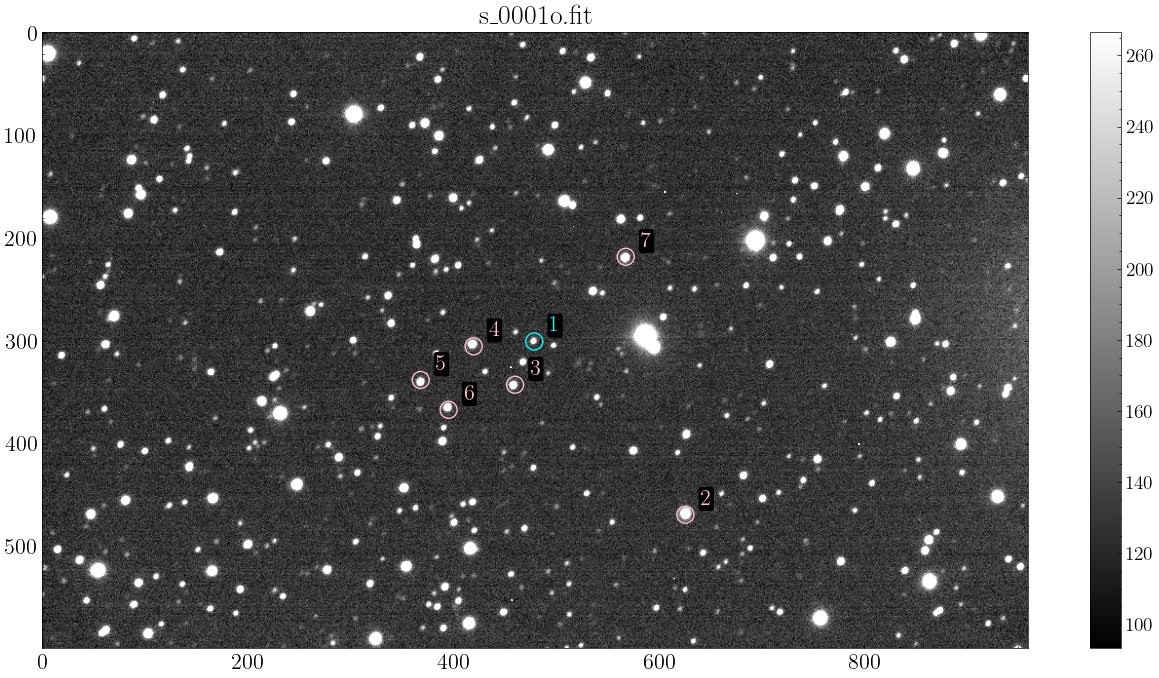
\includegraphics[scale=0.5]{Observaciones/Secciones/Figures/Figura Campo Observado.png}
	\caption{Imagen del campo de \atoObjId marcado con la etiqueta $1$ en, 
	junto a las estrellas de referencia usadas en la fotometría diferencial 
	marcadas en anillos rosas marcados con etiquetas del $2$ al $7$.}
	\label{figuraCcdCampo}
\end{figure}

\subsection{Procesamiento de Imágenes}

La limpieza de las imágenes incluyó la corrección de bias, darks, y flats por
medio de imágenes de calibración, las cuales fueron tomadas cada noche de
observación. Esto fue realizado utilizando tareas standard de IRAF
[\citeyearparen{tody_iraf_1986}]. Cada imagen fue revisada manualmente para
determinar si era de suficiente calidad para hacer una medición adecuada. Se
analizó la forma que proyecta el objeto en la imagen del CCD; solo las imágenes
cuyo perfil se aproxima a un circulo fueron aceptadas para realizar el proceso
de fotometría diferencial.

\begin{figure}[!ht]
	\centering
	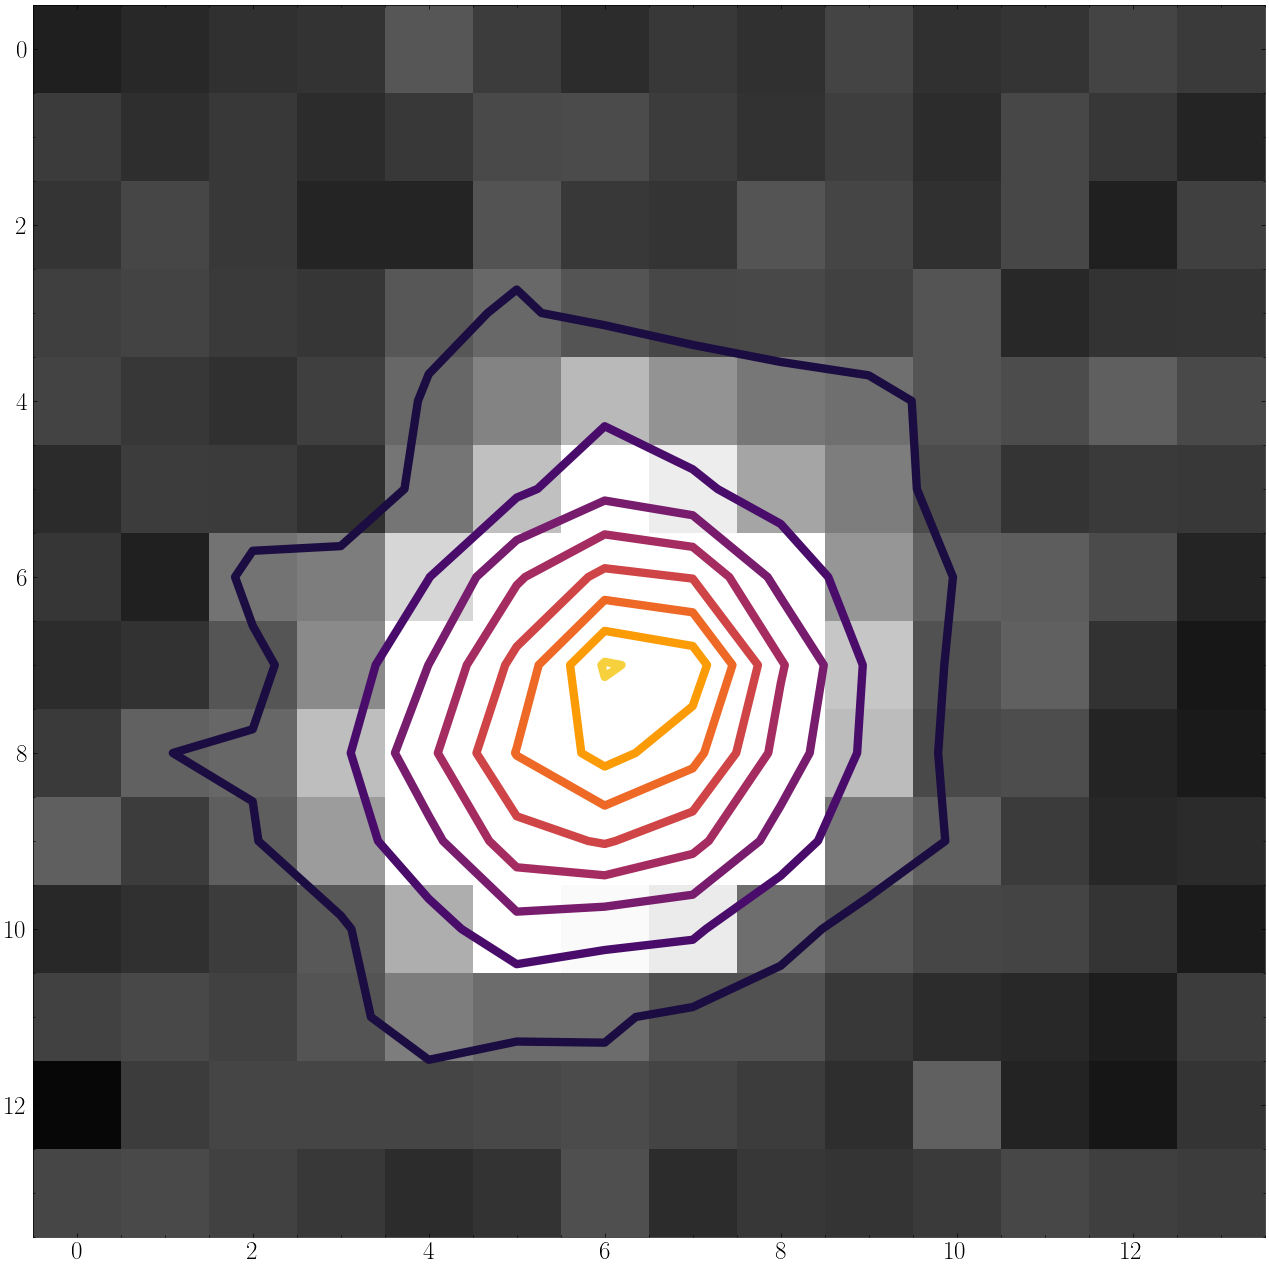
\includegraphics[scale=0.4]{Observaciones/Secciones/Figures/Figura Pixel Perfil Contorno.png}
	\caption{Isógrama de las cuentas registradas del flujo de \atoObjId para un
	corte de $14 \times 14$ pixeles, donde el color más claro denota una mayor
	cantidad de cuentas.}
	\label{figuraPixelContorno}
\end{figure}

Una vez que las mediciones fueran corregidas, fue necesario trasladar los datos
dentro de las imágenes para que \atoObjId quede en el centro del campo,
facilitando la fotometría por apertura. Utilizando el script
\href{https://github.com/KnightIV/UANL_MAPTA_Observaciones/blob/main/analisis/iturbide/shift_images.py}{\code{shift\_images.py}}
se ejecutó una tarea de \textit{plate solving} para cada imagen calibrada; el
proceso de \textit{plate solve}, llevado a cabo utilizando el programa
\textit{Astrometry} [\citeyearparen{astrometry}], toma como referencia estrellas
dentro del campo de la imagen comparando contra una base de datos pre-definida
para determinar las coordenadas físicas que corresponden a una imagen. Esta
información va encapsulada dentro de los metadatos del archivo FITS, conocido
como \textbf{World Coordinate System} (\textbf{WCS}). Una vez que una imagen sea
resuelta se puede proyectar a las coordenadas de otra imagen, posicionando la
estrella variable en una posición única dentro del encuadro de cada imagen,
facilitando el uso de coordenadas en pixeles para definir las aperturas de
medición fotométrica.

Utilizando las imágenes proyectadas se obtuvo el brillo del objeto utilizando
la tarea \code{qphot} de IRAF, dando como resultado magnitudes instrumentales
del sistema. La apertura en tamaño de pixeles se definió en base al ancho a
media altura (\textit{full-width at half-maximum}) de \atoObjId para cada
imagen, utilizando la tarea \code{imexam} de IRAF. Este se usó como el radio de
la apertura circular, junto a una apertura anular para sustraer el brillo de
fondo del cielo, el cual se utilizó para las 7 estrellas marcadas en la
\reffigure{figuraCcdCampo}. Las magnitudes instrumentales medidas se pueden ver
en la \reffigure{figuraCurvaLuzInstrumentalTodas}. A pesar de que todos los
objetos muestran un comportamiento variable, esto no es una característica
intrínseca de todos los sistemas. En particular, la estrella de comparación se
considera que emite un flujo relativamente constante a comparación del sistema
variable \atoObjIdNoSpace; por lo tanto, las variaciones vistas en su curva de
luz se deben a perturbaciones atmosféricas e instrumentales, lo cual nos permite
eliminar estos efectos por medio de la fotometría diferencial.

\begin{figure}[!ht]
	\centering
	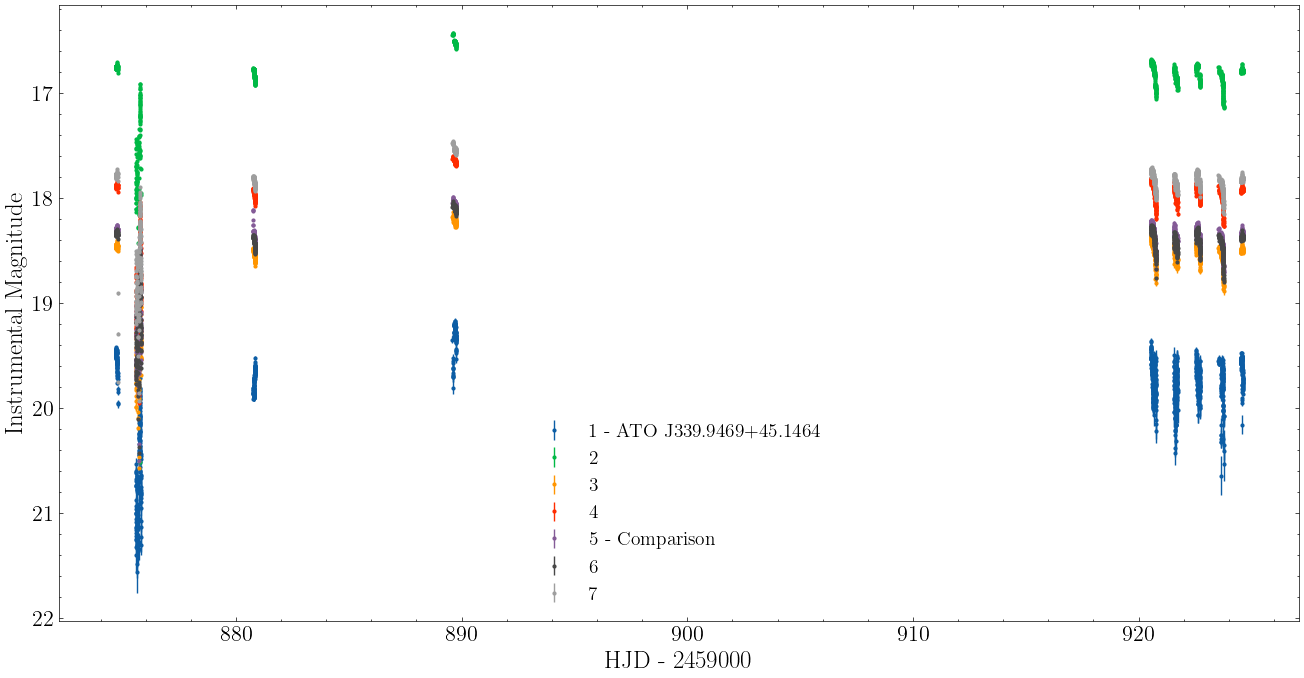
\includegraphics[scale=0.4]{Observaciones/Secciones/Figures/Figura Magnitud Instrumental Todas.png}
	\caption{Magnitudes instrumentales reportada por IRAF mediante la técnica de
	fotometría de apertura. De los 7 objetos resaltados en la
	\reffigure{figuraCcdCampo} se distinguen el objeto principal \atoObjId con
	la etiqueta $1$, y la estrella de referencia utilizada para determinar la
	magnitud diferencial de \atoObjIdNoSpace. }
	\label{figuraCurvaLuzInstrumentalTodas}
\end{figure}

\subsection{Fotometría Diferencial}
Para obtener una magnitud diferencial de \atoObjId se necesita de una estrella
de referencia de la cual se observe un flujo constante. Aparte del requisito de
ser una fuente constante, una estrella de referencia ideal sería del mismo color
que el sistema variable \atoObjIdNoSpace; sin embargo, en casos como el de este
estudio se puede despreciar este último requisito debido al bajo número de
opciones disponibles dentro del campo visible. Del campo visible en la
\reffigure{figuraCcdCampo} se eligió el objeto número $5$ como la estrella de
referencia. Su curva de luz instrumental se puede ver a mayor detalle en la
\reffigure{figuraCurvaLuzInstrumentalReferencia}. La magnitud diferencial $m_d$
de \atoObjId se obtiene restando la magnitud instrumental del objeto de
referencia 5 $m_{\mathrm{inst, 5}}$ de la magnitud instrumental medido de
\atoObjId $m_{\mathrm{inst, \atoObjId}}$ utilizando la
\refequation{ecuacionMagnitudDiferencial}, cuya curva de luz resultante se puede
ver en la \reffigure{figuraIturbideAtoLightCurve}. Las imágenes calibradas se
encuentran como un \textit{Release} dentro del repositorio de GitHub este
proyecto de investigación, junto a los datos de la fotometría de
apertura.\footnote{\url{https://github.com/KnightIV/UANL_MAPTA_Observaciones/releases/tag/data}}

\begin{eqfloat}[!ht]
	\begin{equation}
		m_d = m_{\mathrm{inst, \atoObjId}} - m_{\mathrm{inst, 5}}
	\end{equation}
	\blankcaption
	\vspace{-0.5em}
	\label{ecuacionMagnitudDiferencial}
\end{eqfloat}

\begin{figure}[!ht]
	\centering
	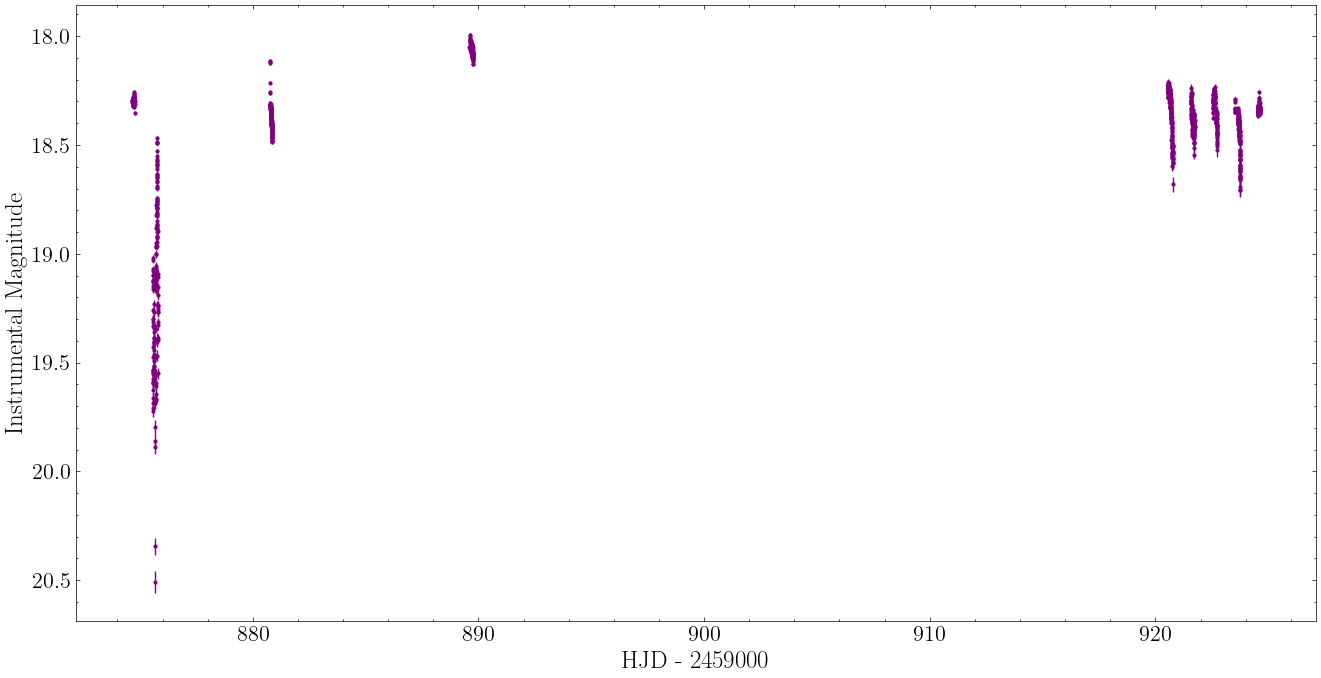
\includegraphics[scale=0.44]{Observaciones/Secciones/Figures/Figura Magnitud Instrumental Estrella Referencia.png}
	\caption{Magnitud instrumental de la estrella de referencia utilizada para
	determinar la magnitud diferencial de \atoObjIdNoSpace. La variabilidad en
	la curva de luz se atribuye a factores extrínsecos del sistema.}
	\label{figuraCurvaLuzInstrumentalReferencia}
\end{figure}

\begin{figure}[!ht]
	\centering
	\xincludegraphics[scale=0.42, label=\textbf{(a)}, labelbox=true, pos=nw, fontsize=\large]{Observaciones/Secciones/Figures/Full LC.png}
	\xincludegraphics[scale=0.34, label=\textbf{(b)}, labelbox=true, pos=nw, fontsize=\large]{Observaciones/Secciones/Figures/Hour Sync LC.png}
	\caption{Magnitud diferencial de \atoObjIdNoSpace. \textbf{(a)} Curva de luz
	completa. \textbf{(b)} Curva de luz segmentada por día, con la cual se logra
	apreciar la cadencia de observación, viendo como cada día se logra observar
	una fase diferente del sistema.}
	\label{figuraIturbideAtoLightCurve}
\end{figure}